\documentclass[letterpaper,  %a4paper
               %boxit,
               %titlepage,   % separate title page
               %refpage      % separate references
              ]{jacow}
%
% CHANGE SEQUENCE OF GRAPHICS EXTENSION TO BE EMBEDDED
% ----------------------------------------------------
% test for XeTeX where the sequence is by default eps-> pdf, jpg, png, pdf, ...
%    and the JACoW template provides JACpic2v3.eps and JACpic2v3.jpg which
%    might generates errors, therefore PNG and JPG first
%
\makeatletter%
	\ifboolexpr{bool{xetex}}
	 {\renewcommand{\Gin@extensions}{.pdf,%
	                    .png,.jpg,.bmp,.pict,.tif,.psd,.mac,.sga,.tga,.gif,%
	                    .eps,.ps,%
	                    }}{}
\makeatother

% CHECK FOR XeTeX/LuaTeX BEFORE DEFINING AN INPUT ENCODING
% --------------------------------------------------------
%   utf8  is default for XeTeX/LuaTeX 
%   utf8  in LaTeX only realizes a small portion of codes
%
\ifboolexpr{bool{xetex} or bool{luatex}} % test for XeTeX/LuaTeX
 {}                                      % input encoding is utf8 by default
 {\usepackage[utf8]{inputenc}}           % switch to utf8

\usepackage[USenglish]{babel}			 
\usepackage{soul}
\usepackage[final]{pdfpages}
\usepackage{multirow}
\usepackage{ragged2e}
\usepackage{tikz}
\usetikzlibrary{shapes.misc}
\usetikzlibrary{shapes,arrows,decorations.markings,shadows,positioning}

%
% if BibLaTeX is used
%
\ifboolexpr{bool{jacowbiblatex}}%
 {%
  \addbibresource{jacow-test.bib}
  \addbibresource{biblatex-examples.bib}
 }{}
\listfiles

%
% command for typesetting a \section like word
%
\newcommand\SEC[1]{\textbf{\uppercase{#1}}}
\newcommand{\lsnote}[1]{\textsf{{\color{violet}{ LS note:}   #1 }}}
\newcommand{\nnnote}[1]{\textsf{{\color{blue}{ NN note:}   #1 }}}
\newcommand{\jlnote}[1]{\textsf{{\color{green}{ JL note:}   #1 }}}
\usepackage{floatrow}
\floatsetup[table]{capposition=top}

%%
%%   Lengths for the spaces in the title
%%   \setlength\titleblockstartskip{..}  %before title, default 3pt
%%   \setlength\titleblockmiddleskip{..} %between title + author, default 1em
%%   \setlength\titleblockendskip{..}    %afterauthor, default 1em

%\copyrightspace %default 1cm. arbitrary size with e.g. \copyrightspace[2cm]

% testing to fill the copyright space
%\usepackage{eso-pic}
%\AddToShipoutPictureFG*{\AtTextLowerLeft{\textcolor{red}{COPYRIGHTSPACE}}}
\graphicspath{ {C:/Users/nneveu/Desktop/emittance_minimization/code/image_scripts} }
\begin{document}

\title{Photoinjector Optimization using a Derivative-Free, Model-Based, 
	Trust-Region Algorithm for the Argonne Wakefield Accelerator } 
	
	%\NoCaseChange{JACoW} conferences\thanks{Work supported by ...}}

\author{N. R. Neveu\textsuperscript{1}\thanks{nneveu@hawk.iit.edu}, J. Larson, J. G. Power, Argonne National Laboratory, Lemont, USA \\
		L. K. Spentzouris, \textsuperscript{1}Illinois Institute of Technology, Chicago, USA}
	
\maketitle

%
\begin{abstract}
% ----------------------------------------------------
Model-based, trust-region, derivative-free algorithms 
are increasingly popular for optimizing computationally 
expensive numerical simulations. A strength of such
methods is their efficient use of function evaluations. 
In this paper, we use one such algorithm to optimize 
the beam dynamics in two cases of interest at the 
Argonne Wakefield Accelerator (AWA) facility. 
First, we minimize the emittance of the electron 
bunch produced by the AWA drive rf photocathode gun 
alone by adjusting three parameters: rf gun phase, 
solenoid strength, and laser radius. The algorithm 
converges to a set of parameters with an
emittance of 1.08 mm-mrad. Second, we expand 
the number of optimization parameters to model 
the complete AWA rf photoinjector linac 
(the gun and six accelerating cavities). 
The optimization algorithm is used in a Pareto study that compares the 
trade-off between beam emittance and bunch 
length for the AWA linac.
\end{abstract}


\section{Optimization Algorithms}
% ----------------------------------------------------
Model-based, derivative-free algorithms are frequently used to optimize
computationally expensive simulations due to their judicious use of function
evaluations. After observing beam properties at
different operational parameters, these methods build models of the unknown
function and then minimize these models to identify candidate parameters to 
evaluate. BOBYQA~\cite{bobyqa} is one such method that is available via the
NLopt~\cite{nlopt} package. Given a candidate minimizer $v^k$, BOBYQA
constructs a quadratic model using function values of points near $v^k$. This
model is minimized near $v^k$ in order to produce a point $v^k + s^k$. If this
point has a better function value than $v^k$, the estimate of the minimum is
updated and a new model is constructed around this new point. If the value at
$v^k + s^k$ is not a sufficient improvement over the value at $v^k$, the model
around $v^k$ is refined.


\section{Code}
% ----------------------------------------------------
To simulate beam dynamics with 3D space charge, 
the open source particle-in-cell code OPAL-T 
\cite{opal} was used. As mentioned in the previous section, 
an open source python package called nlopt \cite{nlopt} was used
in combination with python code written at ANL to perform simulation 
evaluations and minimization. All the files needed to replicate 
the results in this paper are hosted at ZZZZ.com. 
Interested parties are welcome to adapt the code to their needs
and suggest improvements.

\section{The AWA Facility }
% ----------------------------------------------------
The 70 MeV rf photoinjector at the Argonne Wakefield 
Accelerator (AWA) facility  [WEPAB132, these proceedings] 
consists of an rf gun followed by six rf accelerating cavities. 
See Figure~\ref{fig:beamline} for the beam line layout. 
The rf gun [REF] operates at \SI{1.3}{GHz} with three solenoids 
and a Cs2Te photocathode excited by 248 nm UV laser.  
Solendoid 1 (S1) is used to buck the field at the cathode 
while the other two solenoids (S2 and S3) are used for emittance compensation.  
The rf accelerating cavities are 7 cell standing wave 
cavities each with independently controllable phase.

\def \gunleft {-1.2}
\def \gunright {-0.3}

%This should say "left", but I'm lazy and didn't change it
\def \loneright {1.0}
\def \ltworight {3.5}
\def \lthreeright {5.0}
\def \lfourright {7.0}
\def \lfiveright {8.5}
\def \lsixright {10}
\begin{figure*}
	\centering
	\begin{center}
		\begin{tikzpicture}
		%Gun drawings
		\draw[fill=orange, very thick, rounded corners =0.3cm] (\gunleft,0.0)rectangle (\gunright,2) node[pos=.5, white] {\textbf{Gun}} ;
		\draw[ultra thick, fill=black!60!green] (\gunleft-0.45,-1)rectangle  (\gunright-0.45,0) node[pos=.5, white] {\textbf{$S_1, S_2$}} ;
		\draw[ultra thick, fill=black!60!green] (\gunleft-0.45,2)rectangle  (\gunright-0.45,3) node[pos=.5, white] {\textbf{$S_1, S_2$}} ;
		\draw[ultra thick, fill=black!60!green] ({\gunright+0.3},0)rectangle  (0.5,2) node[pos=.5, white] {\textbf{$S_3$}} ;
		
		%Linac drawings 
		\draw[fill=blue, ultra thick, rounded corners =0.2cm] (\loneright,0)rectangle  ({\loneright+1},2) node[pos=.5, white] {L1} ;
		\draw[fill=blue, ultra thick, rounded corners =0.2cm] (\ltworight,0)rectangle  ({\ltworight+1},2) node[pos=.5, white] {L2};
		\draw[fill=blue, ultra thick, rounded corners =0.2cm] (\lthreeright,0)rectangle ({\lthreeright+1},2) node[pos=.5, white] {L3};
		\draw[fill=blue, ultra thick, rounded corners =0.2cm] (\lfourright,0)rectangle ({\lfourright+1},2) node[pos=.5, white] {L4};
		\draw[fill=blue, ultra thick, rounded corners =0.2cm] (\lfiveright,0)rectangle ({\lfiveright+1},2) node[pos=.5, white] {L5};
		\draw[fill=blue, ultra thick, rounded corners =0.2cm] (\lsixright,0)rectangle ({\lsixright+1},2) node[pos=.5, white] {L6};
		
		\draw[very thick] (\gunleft,-1.5) -- (14,-1.5);
		%\path [draw=black, fill=black] (1,-2.5) circle (2pt); %black circle
		%\path [draw=black, fill=white, thick] (2,-2.5) circle (2pt); %white circle
		\draw[latex-latex] (\gunleft,-1.5) -- (14,-1.5) ; 
		\foreach \x in  {0.5, 1.0, 3.5, 5.0, 7.0, 8.5, 10, 12.5} %tick marks
		\draw[shift={(\x,-1.5)},color=black] (0pt,3pt) -- (0pt,-3pt);
		\foreach \x in {0.5, 1.0, 3.5, 5.0, 7.0, 8.5, 10, 12.5}
		\draw[shift={(\x,-1.7)},color=black] (0pt,0pt) node[below] 
		{$\x$};
		
		\node[draw, fill=yellow, star, star points=5, star point ratio=0.6, minimum size=0.6cm]
		at (12.5,1.0) {$z_1$};
		\end{tikzpicture}
	\end{center}
\caption{Layout of the portion of the AWA beam line used as simulation model.}
\label{fig:beamline}
\end{figure*} 


\section{Gun Optimization}
% ----------------------------------------------------
Much work has been done to optimize 1.5 cell rf guns
at \SI{1}{nC} \cite{pitz}. This known solution was used as a test 
of the optimization algorithm BOBYQA \cite{bobyqa}. 
A single objective optimization of emittance, $\epsilon_x$, was 
done over a length of \SI{5}{m}. All linacs were turned off in these simulations. 
Non-varying parameters were based on work done at 
PITZ \cite{pitz}, and a benchmark of OPAL-T, GPT, and ASTRA 
using the AWA's drive gun \cite{benchmark}, see Table~\ref{tab:gun}.
\begin{table}[hbt] %or [hbt] ?
	\centering
	\begin{tabular}{l c c}
		%\toprule
		\textbf{Parameter} & \textbf{Value} \\
		\hline %\midrule
		Charge  & \SI{1}{nC} \\
		Gradient & \SI{60}{MV/m} \\
		Laser FWHM & \SI{20}{ps} \\
		Laser Rise and Fall Time & \SI{6}{ps} \\
		Kinetic Energy at Cathode  & \SI{0.55}{eV} \\
		Buck and Focusing Solenoids & \SI{550}{A}
		%\bottomrule
	\end{tabular}
	\caption{Non-varying Simulation Parameters for Gun Optimization Runs}
	\label{tab:gun}
\end{table}
Three parameters were variable: solenoid strength ($S_3$), gun phase
($\phi_g$), and laser radius (R). Note, phase 
refers to the difference between injection phase and 
phase of max energy gain (on crest). The range for each 
parameter is shown in Table~\ref{tab:parameters}. 
The laser full width half max, T, and cavity phases, $\phi_l$, were added in the 
Pareto front simulations described later. For the 
remainder of the paper, the variables in Table~\ref{tab:parameters} 
will be referred to as $v=\left[S_3, \phi_g, R, T, \phi_l\right]$, where 
$\phi_l=[\phi_{l_1},\,\phi_{l_2},\,\phi_{l_3},\,\phi_{l_4},\,\phi_{l_5},\,\phi_{l_6}]$
represents the phase of each linac cavity 1-6. 
\begin{table}[hbt] %or [hbt] ?
	\centering
	\begin{tabular}{ l *{3}{c}}
		%\toprule
		\textbf{Variable} & \textbf{Range} & \textbf{Unit} \\
		\hline %\midrule
		Solenoid Strength & $ 0 \le S_3 \le 440$  & A \\
		Phase of Gun & $-100^\circ \le \phi_g \le 100^\circ$  & Degrees \\
		Laser Radius & $0.003 \le R \le 0.015$  & m \\
		Laser FWHM & $2 \le T \le $10  & ps \\
		Cavity Phase & $-20 \le \phi_l \le 20$  & MV/m \\
		%\bottomrule
	\end{tabular}
	\caption{Variable Simulation Parameters for Gun and Linac Optimization Runs}	
	\label{tab:parameters}
\end{table}

Optimization runs were started from several points. 
All runs converged to an emittance of 
$\SI{1.08}{\um}$ in less than 100 simulation evaluations. 
An exhaustive search of the parameter space was not done, 
so there may be local minima that were not found.
However, the results match expectations based on literature.

\section{Linac Optimization} 
% ----------------------------------------------------
Next the gun and linac, as shown in Figure~\ref{fig:beamline}, 
was optimized over ten variable parameters, see Table~\ref{tab:parameters}, 
and two objectives: emittance, $\epsilon_x$, and bunch length, $\sigma_z$. 
The location of interest is $z_1=\SI{12.51}{m}$, 
as this is the entrance of the first 
quad after the last accelerating cavity. 
We choose to optimize $\epsilon_x$
instead of $\epsilon_{xy}$, because 2D field maps were 
used for the rf cavities, with no appreciable 
difference between the resulting x and y values.

The non-varying parameters for all 
linac simulation runs are shown in Table~\ref{tab:linac}.
The initial kinetic energy parameter is missing because a different
emission model was used in this case. OPAL-T has the 
ability to model emission based on cathode material and laser
properties. This method was used to simulate emission
from a CsTe cathode using a laser with initial kinetic energy of 4 eV. 
These are typical operating conditions at AWA. 
\begin{table}[hbt] %or [hbt] ?
	\centering
	\begin{tabular}{l c c}
		%\toprule
		\textbf{Parameter} & \textbf{Value} \\
		\hline %\midrule
		Charge  & \SI{40}{nC} \\
		Laser Rise and Fall Time & \SI{1.0}{ps} \\
		Gun Gradient & \SI{70}{MV/m} \\
		Buck and Focusing Solenoids & \SI{550}{A}\\
		Cavity Gradient 1-4 & \SI{25}{MV/m} \\
		Cavity Gradient 5-6 & \SI{27}{MV/m} \\
		
		%\bottomrule
	\end{tabular}
	\caption{Non-varying Simulation Parameters for Linac Optimization Runs}
	\label{tab:linac}
\end{table}

A 1,000 point sample of linac parameters were drawn uniformly from the domain
in Table~\ref{tab:parameters} and evaluated. 132 of these simulations completed
without error. The emittance and bunch length at $z_1=\SI{12.51}{m}$ was
calculated. These values allow us to produce shifted and scaled emittance
and bunch length ($\bar{\epsilon}_x$, $\bar{\sigma}_z$) that both have a
minimum value of 0 and a maximum value of 1 over the 132 point sample set.
This scaling is done to remove differences in the units of emittance and bunch length
when optimizing.

With these scaled objectives, we then solve a sequence of eleven optimization problems
by minimizing 
\begin{equation}
  f(v,w) = w \bar{\epsilon}_x(v,z_1) + (1-w) \bar{\sigma}_z(v,z_1),
\label{eq:newobj}
\end{equation}
for each $w \in \left\{ 0,0.1,\ldots,1 \right\}$. For each weight $w$, BOBYQA
was started from the sample point with the smallest value of $f(v,w)$.  This
resulted in six unique starting points instead of eleven because, for example, sample number 18
had the smallest value of $f(v,0.5)$, $f(v,0.6)$, and $f(v,0.7)$.

\jlnote{Nicole, I think we may want to consider starting more runs\ldots}
\section{Pareto Front for Linac} 
% ----------------------------------------------------
Figure \ref{fig:pareto} shows the sample points, 
weighted starting points, and resulting Pareto front.
It is clear that BOBYQA improved both emittance and bunch 
length for each of the weighted points. 
The amount of evaluations needed to obtain each Pareto point 
varied from a minimum of 112 evaluations to a maximum of 208 
evaluations. To generate every point in Fig. \ref{fig:pareto}, 
a total of 2215 simulation evaluations.\nnnote{will need to add in w0 and w5 evals when finished}
BOBYQA's progress per iteration for each weight is shown in 
Fig. \ref{fig:iterations}. The convergence criteria was set to 1e-4.  

\begin{figure}[h]
	\centering
	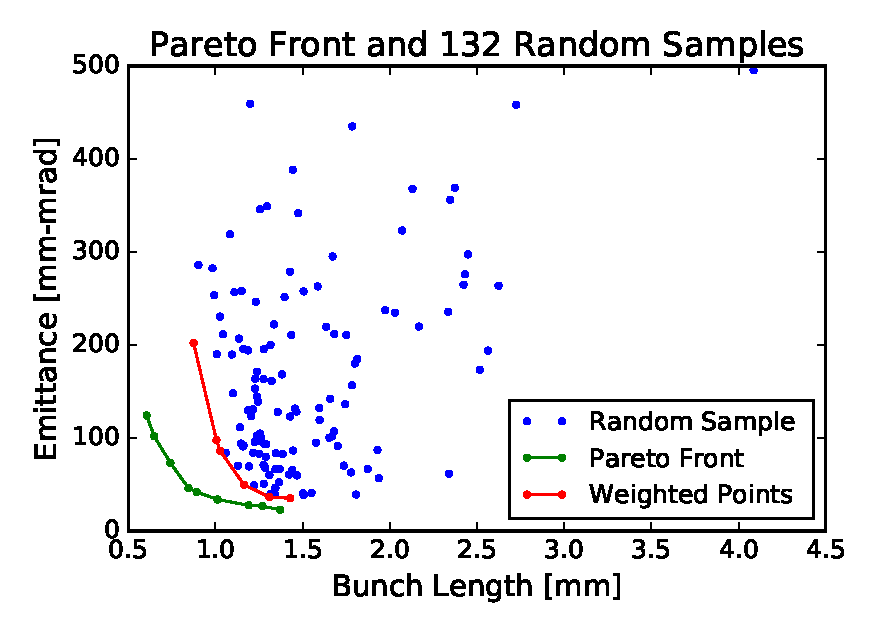
\includegraphics[width=1.0\textwidth]{../../image_scripts/pareto_emittance_vs_zrms}
	\caption{Random sample results, weighted starting points, and resulting Pareto front.}
	\label{fig:pareto}
\end{figure}

\begin{figure}[h]
	\centering
	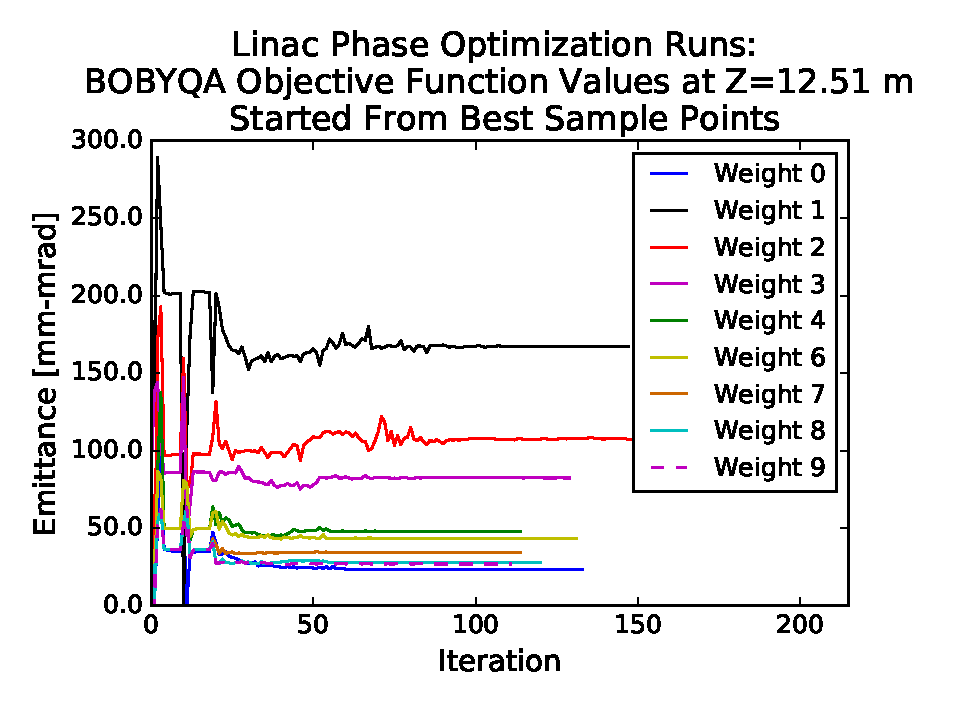
\includegraphics[width=1.0\textwidth]{../../image_scripts/BOBYQA_objective_function_values_linac_10optvariables_10runs_RandSampleGrid1}
	\caption{Amount of iterations needed before converging to tolerance of 1e-4.}
	\label{fig:iterations}
\end{figure}

\section{Conclusion and Future Work}
% ----------------------------------------------------
Using an AWA beam line as the model, BOBYQA
was used to optimize the gun and linac. A Pareto front 
comparing the trade-off between bunch length and emittance
was generated for the linac. Future work will include
refinement of results using 3D field files for all 
cavities, experimental measurements to verify the 
Pareto front, and comparison to genetic algorithms.

\section{Acknowledgment}
% ----------------------------------------------------
We gratefully acknowledge the computing resources
provided on Blues, a high-performance computing cluster
operated by the LCRC at Argonne National Laboratory.
This material is based upon work supported by the 
U.S. Department of Energy, Office of Science, under 
contract numbers DE-AC02-06CH11357, DE-AC02-06CH11357, 
and grant number DE-SC0015479. 

% ----------------------------------------------------
\bibliographystyle{plain}
\bibliography{../../bibs/masterbib}
\end{document}
	
